\documentclass[a4paper, 12pt, titlepage]{article}


% Geometry package, setting margin.
\usepackage[top=2.5cm, bottom=2.5cm, left=2.5cm, right=2.5cm]{geometry}
\usepackage{multicol}

% Enum control.
\usepackage{enumerate}

% Hyperlink
\usepackage[
    pdfstartview=FitH,
    CJKbookmarks=true,
    bookmarks=true,
    bookmarksnumbered=true,
    bookmarksopen=true,
    colorlinks=true,
    citecolor=black,
    linkcolor=black,
    anchorcolor=black,
    urlcolor=black
]{hyperref}

% Title format
\usepackage{titlesec}
% List of figure, table, etc.
\usepackage{titletoc}
% Table control
\usepackage{booktabs}
% Appendix control
\usepackage[title,titletoc,header]{appendix}

% Font size control
\usepackage{type1cm}
% Indentation control
\usepackage{indentfirst}
\usepackage{changepage}

% Color control
\usepackage{color,xcolor}

%% AMS LaTeX
\usepackage{amsmath,amssymb}
\usepackage{latexsym,textcomp}

%% By Xiao Hanyu
%% 数学公式中的黑斜体
% \usepackage{bm}

%% By Xiao Hanyu
%% 调整公式字体大小:\mathsmaller, \mathlarger
% \usepackage{relsize}

% graphics
\usepackage{graphicx}
\usepackage{subfig}
\usepackage{indentfirst}
\usepackage{float}
\usepackage{url}

% pgf/tikz graph
\usepackage{pgf,tikz}
\usetikzlibrary{shapes,automata,snakes,backgrounds,arrows}
\usetikzlibrary{mindmap}

\usepackage{fancyhdr}
\pagestyle{plain}

%% By Xiao Hanyu
%% 有时会出现\headheight too small的warning
\setlength{\headheight}{15pt}

% Source code
\usepackage{listings}
% Algorithm
\usepackage[ruled,vlined]{algorithm2e}
% Tree graph
\usepackage{synttree}

\usepackage{multirow}

% Source code settings
\lstloadlanguages{}
\lstset{
showstringspaces=false,              %% 设定是否显示代码之间的空格符号
numbers=left,                        %% 在左边显示行号
numberstyle=\tiny,                   %% 设定行号字体的大小
basicstyle=\footnotesize,            %% 设定字体大小\tiny, \small, \Large等等
keywordstyle=\color{blue!70}, commentstyle=\color{red!50!green!50!blue!50},
                                     %% 关键字高亮
frame=shadowbox,                     %% 给代码加框
rulesepcolor=\color{red!20!green!20!blue!20},
escapechar=`,                        %% 中文逃逸字符,用于中英混排
xleftmargin=2em,xrightmargin=2em, aboveskip=1em,
breaklines,                          %% 这条命令可以让LaTeX自动将长的代码行换行排版
extendedchars=false                  %% 这一条命令可以解决代码跨页时,章节标题,页眉等汉字不显示的问题
}

%% 一号, 1.4倍行距
\newcommand{\yihao}{\fontsize{26pt}{36pt}\selectfont}
%% 二号, 1.25倍行距
\newcommand{\erhao}{\fontsize{22pt}{28pt}\selectfont}
%% 小二, 单倍行距
\newcommand{\xiaoer}{\fontsize{18pt}{18pt}\selectfont}
%% 三号, 1.5倍行距
\newcommand{\sanhao}{\fontsize{16pt}{24pt}\selectfont}
%% 小三, 1.5倍行距
\newcommand{\xiaosan}{\fontsize{15pt}{22pt}\selectfont}
%% 四号, 1.5倍行距
\newcommand{\sihao}{\fontsize{14pt}{21pt}\selectfont}
%% 半四, 1.5倍行距
\newcommand{\bansi}{\fontsize{13pt}{19.5pt}\selectfont}
%% 小四, 1.5倍行距
\newcommand{\xiaosi}{\fontsize{12pt}{18pt}\selectfont}
%% 大五, 单倍行距
\newcommand{\dawu}{\fontsize{11pt}{11pt}\selectfont}
%% 五号, 单倍行距
\newcommand{\wuhao}{\fontsize{10.5pt}{10.5pt}\selectfont}

%% 中文破折号,据说来自清华模板
\newcommand{\pozhehao}{\kern0.3ex\rule[0.8ex]{2em}{0.1ex}\kern0.3ex}

%% 设定段间距
\setlength{\parskip}{0.5\baselineskip}
%% 设定行距
\linespread{1}
%% 设定itemize环境item的符号
\renewcommand{\labelitemi}{$\bullet$}

% Begin mathematical commands
\newcommand{\R}{\mathbb{R}}
\newcommand{\Z}{\mathbb{Z}}
\newcommand{\N}{\mathbb{N}}
\newcommand{\Q}{\mathbb{Q}}
\newcommand{\F}{\mathcal{F}}

\newcommand{\Rev}{\textsc{Rev}}
\newcommand{\SRev}{\textsc{SRev}}
\newcommand{\BRev}{\textsc{BRev}}

\newcommand{\E}{\mathbb{E}}
\newcommand{\D}{\mathbb{D}}
\newcommand{\ER}{\mathrm{ER}}

\newcommand{\ud}{\mathrm{d}}
\newcommand{\real}{\mathrm{Re}}
\newcommand{\imag}{\mathrm{Im}}

\newcommand{\KL}{\mathrm{KL}}

\newcommand{\Infer}{\Rightarrow}

% Begin CJK
\usepackage{xltxtra,fontspec,xunicode}

%% \CJKsetecglue{\hskip 0.15em plus 0.05em minus 0.05em}
%% slanfont: 允许斜体
%% boldfont: 允许粗体
%% CJKnormalspaces: 仅忽略汉字之间的空白,但保留中英文之间的空白。
%% CJKchecksingle: 避免单个汉字单独占一行。
\usepackage[slantfont, boldfont]{xeCJK}

% Chinese line break strategy
\XeTeXlinebreaklocale "zh"
\XeTeXlinebreakskip = 0pt plus 1pt minus 0.1pt

% 设置中文标点样式,支持quanjiao、banjiao、kaiming等多种方式
\punctstyle{kaiming}

% Default Chinese font
\setCJKmainfont[BoldFont={Adobe Heiti Std}, ItalicFont={Adobe Kaiti Std}]{Adobe Song Std}
% Chinese sans font
\setCJKsansfont[BoldFont={Adobe Heiti Std}]{Adobe Kaiti Std}
% Chinese mono font
\setCJKmonofont{Adobe Heiti Std}

% English sarif font
\setmainfont{DejaVu Serif}
% English sans font
\setsansfont{DejaVu Sans}
% English mono font
\setmonofont{DejaVu Sans Mono}

% CJK fonts
\setCJKfamilyfont{song}{Adobe Song Std}
\setCJKfamilyfont{kai}{Adobe Kaiti Std}
\setCJKfamilyfont{hei}{Adobe Heiti Std}
\setCJKfamilyfont{fangsong}{Adobe Fangsong Std}
\setCJKfamilyfont{lisu}{LiSu}
\setCJKfamilyfont{youyuan}{YouYuan}

%% 自定义宋体
\newcommand{\song}{\CJKfamily{song}}
%% 自定义楷体
\newcommand{\kai}{\CJKfamily{kai}}
%% 自定义黑体
\newcommand{\hei}{\CJKfamily{hei}}
%% 自定义仿宋体
\newcommand{\fangsong}{\CJKfamily{fangsong}}
%% 自定义隶书
\newcommand{\lisu}{\CJKfamily{lisu}}
%% 自定义幼圆
\newcommand{\youyuan}{\CJKfamily{youyuan}}

% Begin mathematical envs
\newtheorem{example}{例}
\newtheorem{problem}{问题}
\newenvironment{proof}{\noindent\textbf{证明\ }}{\hspace*{\fill}$\Box$\medskip}
\newenvironment{solution}{\noindent\textbf{解答\ }}{\hspace*{\fill}$\Box$\medskip}
\newtheorem{algo}{算法}

\newtheorem{definition}{定义}
\newtheorem{axiom}{公理}
\newtheorem{theorem}{定理}
\newtheorem{lemma}{引理}
\newtheorem{corollary}{推论}

\newtheorem{property}{性质}
\newtheorem{proposition}{命题}
\newtheorem{remark}{注解}
\newtheorem{condition}{条件}
\newtheorem{assumption}{假设}
\newtheorem{conclusion}{结论}

% Section title
\renewcommand{\contentsname}{目录}
\renewcommand{\abstractname}{摘要}
\renewcommand{\indexname}{索引}
\renewcommand{\listfigurename}{插图目录}
\renewcommand{\listtablename}{表格目录}
\renewcommand{\figurename}{图}
\renewcommand{\tablename}{表}
\renewcommand{\algorithmcfname}{算法}
\renewcommand{\appendixname}{附录}
\renewcommand{\appendixpagename}{附录}
\renewcommand{\appendixtocname}{附录}
\renewcommand\refname{参考文献}
% \renewcommand\bibname{参考文献}

% Section title format
\titleformat{\chapter}{\centering\huge}{第\thechapter{}章}{1em}{\textbf}
\titleformat{\section}{\centering\sihao}{\thesection}{1em}{\textbf}
\titleformat{\subsection}{\xiaosi}{\thesubsection}{1em}{\textbf}
\titleformat{\subsubsection}{\xiaosi}{\thesubsubsection}{1em}{\textbf}


\begin{document}
%% 中文习惯是设定首行缩进为2em. 注意此设置一定要在document环境之中, 这可能与\setlength作用范围相关 
\setlength{\parindent}{2em}

\title{基于立体视觉与末端摄像头的\\机械臂准确抓取系统}
\author{清华大学第三十四届“挑战杯”\\学生课外学术科技作品竞赛正式文档}
\date{}
\maketitle

\section*{摘要}

家庭机器人是机器人发展的一大方向,但目前主流的家庭机器人无法抓取物品,更难以进行生活中其他常见的对物体的操作。\ 本文从机械臂出发,提出并设计实现了一套适用于室内环境的抓取系统,结合立体视觉与末端摄像头,使用针对室内场景优化的视觉算法定位物体、识别物体,并引导机械臂进行准确的抓取。\ 另外,为了增加机械臂的使用范围,我们为机械臂增加升降台与移动底盘,让机械臂能够在室内自由的移动,取放更大范围内的物体。\ 本项目经过大量实验,验证了抓取系统在实际生活场景中的适应能力。

\textbf{关键字:}视觉伺服,物体识别,立体视觉

\newpage

\tableofcontents
% \listoffigures
% \listoftables

\section{项目背景}

随着智能化控制的进步,工业4.0时代逐渐到来,智能制造与智能家居产业发展迅速,机器人也慢慢走近每家每户。\ 目许多家庭中配备了扫地机器人用来自动清扫地面,让人在每天忙碌的工作后不必再面对扫地的烦恼。\ 智能家庭机器人Jibo能够识别人的情感并与人产生交互,为家庭生活平添了一份乐趣。\ 而在未来,智能家居机器人可能成为家庭的一员,完成更加复杂的任务,辅助人们日常的工作、学习、娱乐,替代人类完成繁杂、琐碎的家务活。\

\begin{figure}[H]
\begin{minipage}[t]{0.5\textwidth}
	\centering
    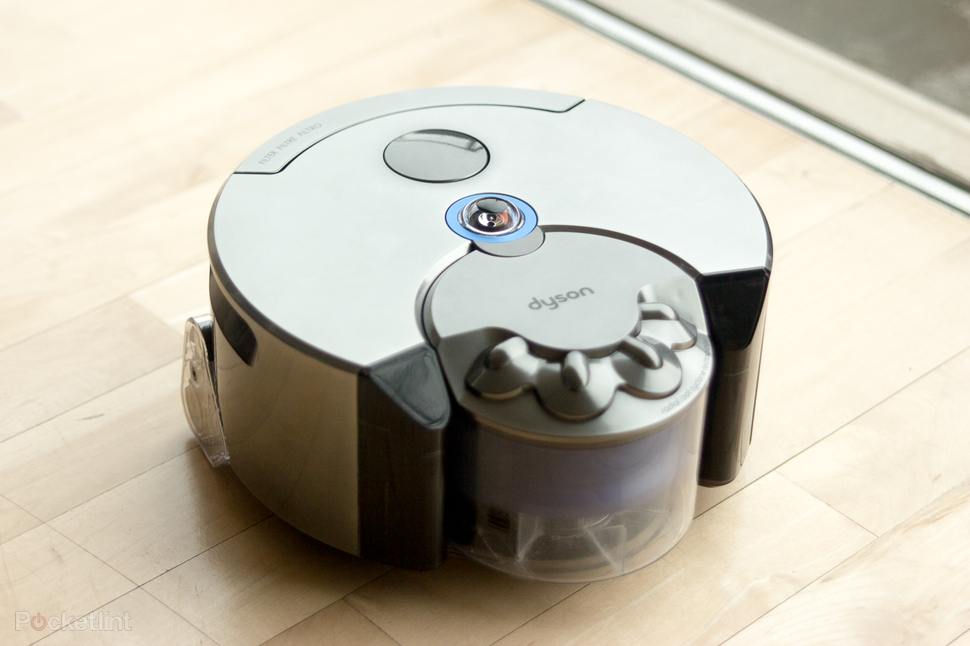
\includegraphics[width = 0.8\textwidth]{pictures/dyson.jpg}
    \caption{Dyson扫地机器人}
    \label{fig:dyson}
\end{minipage}
\begin{minipage}[t]{0.5\textwidth}
	\centering
    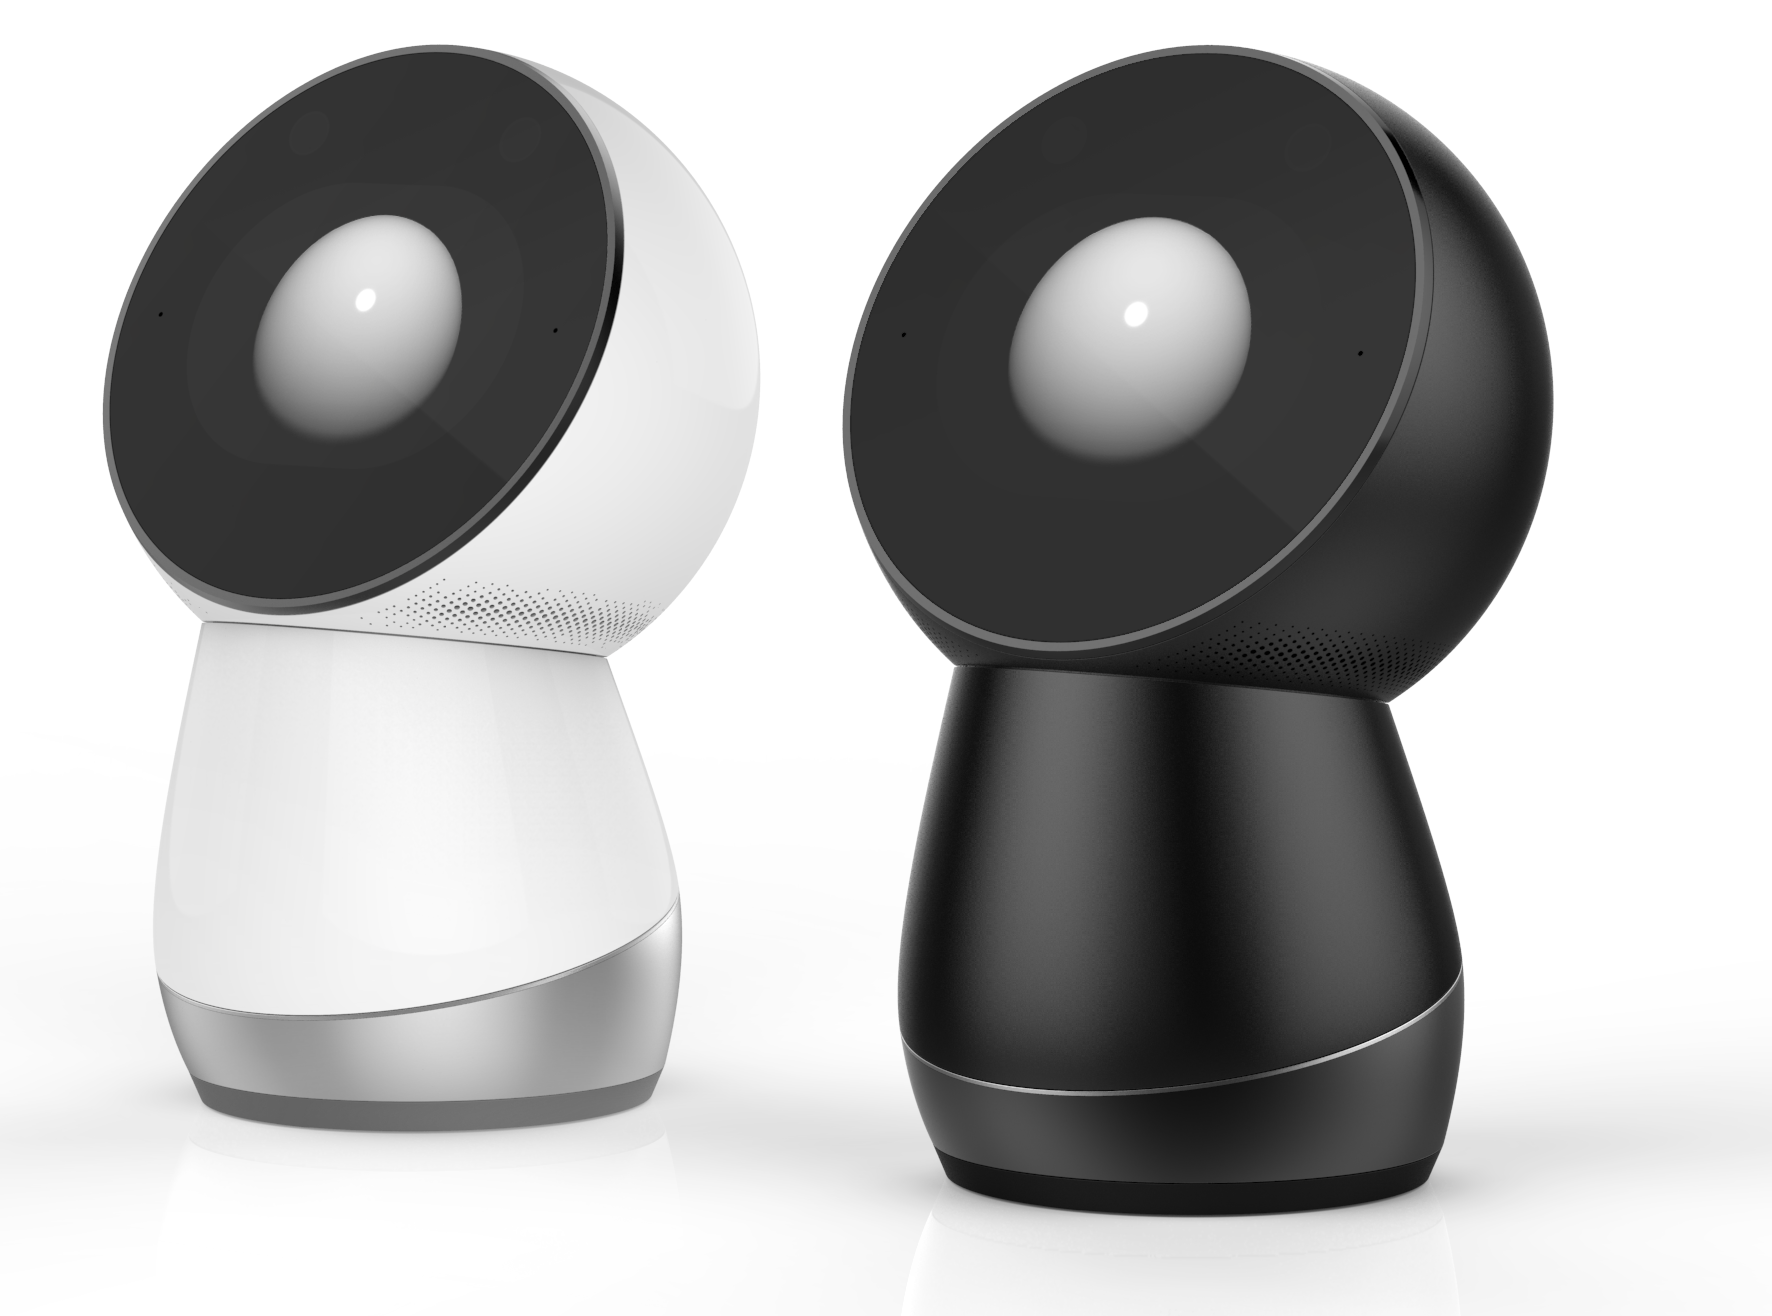
\includegraphics[width = 0.8\textwidth]{pictures/jibo.png}
    \caption{Jibo家庭机器人}
    \label{fig:jibo}
\end{minipage}
\end{figure}

目前,市场上大多数的家庭机器人还都停留在小型的阶段,虽然在软件上已经达到了能感知环境、理解情感、流畅交流的程度,但仍然无法摆脱自身硬件方面的限制,不能帮助完成许多日常生活中看似简单的任务。\ 我们在日常生活中最基本的操作就是拿取物品,而小型的机器人由于体型过小或没有可移动部分,无法做出这些动作,更不可能做出把一个指定的东西送到手边、整理桌上杂乱物品这类更加复杂的动作。\ 另外,目前的智能电器大多只是一个个分立的器件,无法构成一个整体,给人造成了许多的不方便。\ 比如,智能洗衣机在洗完衣服后仍然需要人去晾衣服,智能冰箱也还需要人去开门拿食材。\ 这些“最后一步”的问题也让智能家居的体验大打折扣。\ 

因此,我们希望实现一个可以移动的机械臂,能够在日常的生活场景中自动识别并抓取、放置物体,连接人与物品,连接人与家居。\ 它能从摆放了各种物品的柜子上帮你取下指定的那一个,或者把桌上杂乱的物体排列整齐。\ 基本的物体操纵功能在实际生活中使用十分广泛,我们的机械臂也将胜任日常生活中的大部分任务,能帮人大大减轻负担。\ 

\section{项目创新点}

% 机械臂自动抓取在工业与民用领域都有着广泛的应用。\ 在工业上,由于机械臂工作环境固定,故多采用预先编程、开环控制的方式,不能够适应复杂多变的现实环境。\ 另外,也多采用视觉与机械臂分离的方式,在流水线的一个环节中使用机器视觉进行识别,下一个环节通过机械臂姿态解算来抓取物体,整体的集成度不高。

% 对于更加复杂多变的民用场景,也不乏对于机械臂物体操纵的研究。\ 
在复杂多变的现实场景中,机械臂自动抓取的任务较为困难,但目前已经有一些研究成果。\ 瑞士洛桑联邦理工学院的LASA实验室使用能获取关节角度信息的轻量级机械臂KUKA,经过手动训练,通过外部相机的视觉信息能准确抓取飞行中的物体\cite{kim2014catching}。\ 卡内基梅隆大学NREC部门的ARM-S机器人利用三维传感器获得场景点云并提取识别物体,采用关节反馈来准确获得机械臂的位置\cite{nrec}。\ 这些机械臂都内置了关节反馈,对电机精度也提出了较高的要求,导致机械臂制造成本较高。\ 另外,由于缺少机械臂的末端视觉反馈,机械臂在移动时使用开环控制,难以应对现实场景中突发的变化。

为此,我们提出了一套抓取系统,利用灰度熵与准对室内场景优化的算法来分离物体,使用基于稀疏表示的分类器来识别物体,采用末端视觉反馈来引导机械臂的抓取。这套结合了多种算法的系统能够很好地完成室内环境的物品抓取任务。\ 具体创新点如下。

\subsection{使用末端视觉进行视觉伺服}

我们的机械臂最基础的功能就是抓取物体,而在复杂的室内环境中,通过深度视觉获取到的物体位置信息不够准确,加上机械臂本身的旷量与电机角度的误差,若用开环控制机械臂的移动,很容易导致抓取的不准确,还有可能让机械手触碰到附近的其他物体。\ 

为了解决这一问题,我们在机械手上加装了末端摄像头,使用基于图像的视觉伺服(Image-Based Visual Servoing),构成一个手眼(eye-in-hand)机械臂系统,通过末端视觉获得的物体位置作为反馈,构成机械臂移动的闭环控制,保证物体的准确抓取。\ 

\subsection{物体分辨与识别}

物体识别的一般方法是通过计算两个矩阵的标准化降采样矩阵的点击来判断相似性\cite{aldoma2012point},这样做虽然有一定的效果,但结果的点积值却没有实际意义,对于不同的物体相差非常大,因此难以取合适的阈值,判断的鲁棒性不高。\ 

我们采用了基于稀疏表示的分类器来解决这一问题。首先,我们假设当样本数量足够时,每张该物体的照片都可以近似表示为该物体样本照片的线性叠加。随后,使用稳定$L_1$范数最小化问题估算稀疏解,通过残差来确定识别结果。使用这种方式,算法的鲁棒性有了显著的提升,同时速度和存储空间利用效率上并没有显著的降低。\ 

\subsection{灰度熵分离前后景}

在项目的实践过程中,我们需要一种方法,实时地在以书架为背景的典型场景中,找到所有目标物体的三维坐标。\ 已知的目标查找方法有很多,但鉴于环境的复杂性和图片的质量,已知的算法很难在很短的时间内完成标记目标的任务。\ 

我们针对书架场景的特点提出了基于熵过滤的目标查找算法。\ 首先使用灰度熵的方法过滤背景,但对于纯色物体与书架边框区域会产生误判。\ 作为弥补,我们又提出了目标纯色快提取方法和线段检测方法,分别查找纯色物体和过滤书架框架。\ 利用过滤结果,配合Kinect获取得到的深度信息,再配合三维墙面提取、欧几里得聚类,最终可以确定每一个物体的三维坐标。\ 


\section{项目内容}

\subsection{整体架构}

\subsubsection{系统整体架构}
系统的主要由以下部分构成:
\begin{enumerate}
    \item 运行于主计算机ROS(机器人操作系统)上的算法与决策层
    \item 运行于Xilinx ZYNQ 7020芯片上的ROS系统的上的硬件接口层, 用于对主计算机难以直接控制的硬件进行信号采集和驱动
    \item 深度摄像头Kinect, 用于初步的物体识别
    \item 机械臂, 用于物体抓取
    \item 机械臂末端摄像头与超声波传感器,用于末端的目标位置修正与反馈
    \item 机器人移动平台,用于扩展机械臂的抓取范围
\end{enumerate}

各个部分之间的连接方式如图\ref{fig:structure}所示。\ 
\begin{figure}[ht]
    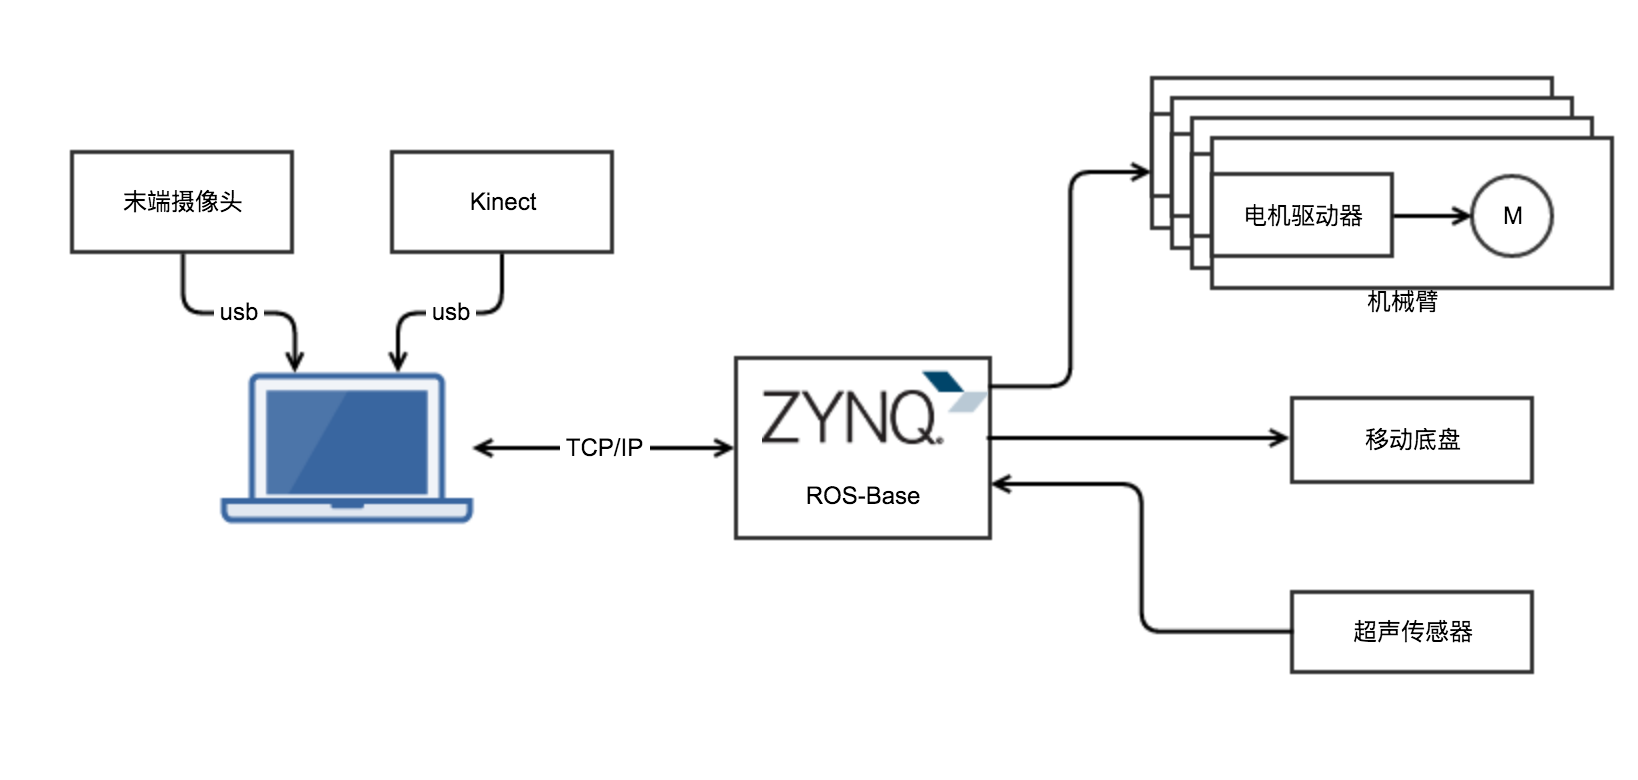
\includegraphics[width = \textwidth]{images/arch.png}
    \caption{整体系统架构}
    \label{fig:structure}
\end{figure}

\subsubsection{通信架构设计思路}
系统整体的硬件通信架构基于机器人操作系统ROS构建。\ ROS是一个基于网络协议的通信系统,支持分布式的节点。\ 
在主机器人上运行的节点负责图像处理与机械臂的运动规划。\ 规划的结果通过网络发送到同样运行着ROS的ZYNQ芯片上。\ 
ZYNQ芯片是一种同时集成了ARM微处理器和FPGA可编程逻辑的全可编程器件。\ 在FPGA上构建了用于直接控制电机并且采集超声波传感器反馈的外设。\ 
而在微处理器上运行的ROS节点通过网络从主计算机运行的ROS节点上收到控制机械臂姿态目标,转换为实际电机的PWM脉宽写入电机控制外设。\ 
同时另一个ROS节点采集超声反馈信息通过网络发送到主计算机上用于之后的运动规划。\ 

\subsubsection{视觉系统设计思路}
Kinect深度摄像头可以给出0.6m到4.5m之内的立体图像。\ 通过图像处理方法分辨出深度图像中的物体。\ 然而由于Kinect深度摄像头本身的分辨率和净度所限,会产生深度和位置信息不准确以及误报物体等情况。\ 

为了修正这些误差,我们使用了一个机械臂末端的摄像头。\ 主计算机从末端摄像头图像中提取出可能的物体区域,和预先采集的物品图像库进行匹配。\ 如果匹配失败,就认为该物品为Kinect误报。\ 如果匹配成功就开始物品的抓取,在抓取过程中利用末端摄像头看到的物品图像进行反馈。\ 反馈目标为将物品图像定位到末端摄像头图像的中心,同时通过超声波传感器信息采集机械手到物体的距离就可以达到准确抓取的效果。\ 

实际抓取过程的详细流程图如图\ref{fig:flowchart}所示。\ 

\begin{figure}
	\centering
    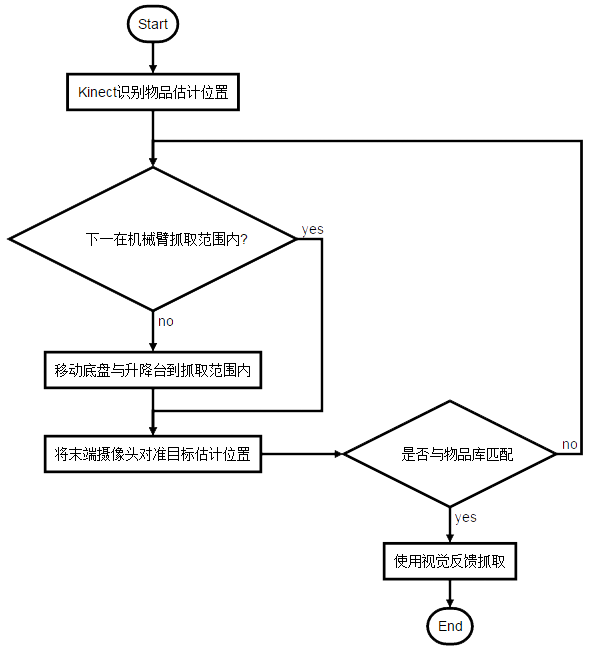
\includegraphics[width = 0.9\textwidth]{images/flow.png}
    \caption{抓取流程图}
    \label{fig:flowchart}
\end{figure}

\subsubsection{坐标定义}

在整个抓取过程中使用的坐标定义如下:
\begin{enumerate}
    \item 机器人本体坐标系 base\_link, 以机器人正前方为x轴,正左方为y轴的右手系
    \item Kinect坐标系 kinect\_link,以kinect正左方为x轴,正上方为y轴的右手系
    \item 末端视觉坐标系 hand\_link,以机械手正前方为x轴,正左方为y轴的右手系
\end{enumerate}

\subsection{项目设计及实现细节}
\subsubsection{图像处理}
\paragraph{灰度熵}

以图\ref{fig:registered}为例,我们将演示分离书架上的物体和书架的算法。\ 直接利用灰度熵,去除书架背景,结果如图\ref{fig:entropy_block}所示。\ 对于一张给定的图片,其熵的定义如下:
\begin{equation}
	E = -\Sigma p_{i} \cdot \log_{2}p_{i}
\end{equation}

\begin{figure}[H]
\begin{minipage}[t]{0.5\textwidth}
	\centering
    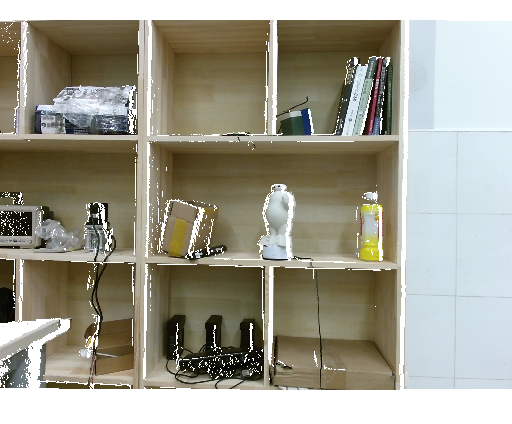
\includegraphics[width = 0.8\textwidth]{images/registered.png}
    \caption{示例图片}
    \label{fig:registered}
\end{minipage}
\begin{minipage}[t]{0.5\textwidth}
	\centering
    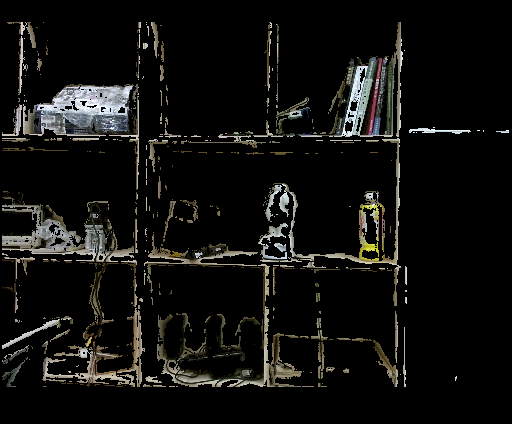
\includegraphics[width = 0.8\textwidth]{images/entropy_block.png}
    \caption{灰度熵结果}
    \label{fig:entropy_block}
\end{minipage}
\end{figure}

在这张图片中,书架被过滤得很干净。\ 不过那些纯色的物体也被过滤了。\ 此外,书架的框架也没有去除干净,所以这张图片还不能用于目标的定位和识别。\ 针对熵过滤的不足,我们又提出了色块检测、线段检测方法。\     
    
\paragraph{色块检测}

在图片进行边缘检测之后,降采样,找到其中的纯色块。\ 其中位于边缘部分的色块意义不大,直接忽略,结果如图\ref{fig:downsampled_filled}。\ 

\begin{figure}[H]
\begin{minipage}[t]{0.5\textwidth}
	\centering
    
\includegraphics[width = 0.8\textwidth]{images/downsampled_filled.png}
    \caption{色块检测结果}
    \label{fig:downsampled_filled}
\end{minipage}
\begin{minipage}[t]{0.5\textwidth}
	\centering
    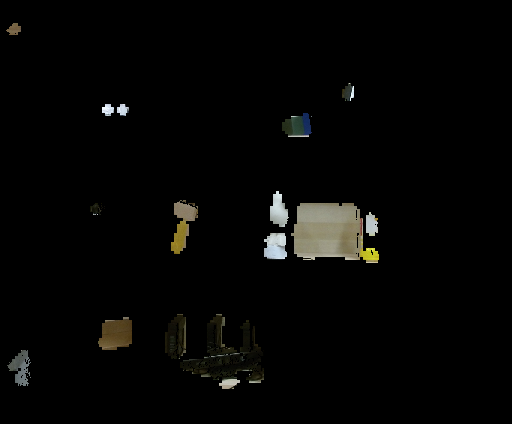
\includegraphics[width = 0.8\textwidth]{images/color_block.png}
    \caption{色块分离结果}
    \label{fig:color_block}
\end{minipage}
\end{figure}

这些色块中,既有背景色块,又有目标色块,需要将他们分离。\ 首先,将剩余色块中面积最大的色块视为标准背景色块(如果标准背景色块的面积比较小,则认为所有色块均为目标色块,终止背景色块识别操作)。\ 检查所有色块,面积同标准背景色块相近、或者颜色同标准背景色块类似的色块,均被视为背景色块。\ 其余的部分直接视作目标色块。\ 最后,将降采样的结果重新应用到图片上,获得图片的色块层,如图\ref{fig:color_block}。\ 

可以观察到色块检测也存在缺陷,在背景颜色起伏较大的细节区域可能无法准确辨别背景色块和目标色块。\ 这些区域将会在平面检测时过滤。\ 

\paragraph{线段检测}

在图片进行边缘检测之后,降采样,如图\ref{fig:raw_contour}所示。\ 将边缘点过分密集的区域清理掉,这些特征点密集的区域应当是目标,结果如图\ref{fig:after_contour}。\ 	
\begin{figure}[H]
\begin{minipage}[t]{0.5\textwidth}
	\centering
    
\includegraphics[width = 0.8\textwidth]{images/raw_contour.png}
    \caption{边缘检测结果}
    \label{fig:raw_contour}
\end{minipage}
\begin{minipage}[t]{0.5\textwidth}
	\centering
    
\includegraphics[width = 0.8\textwidth]{images/after_contour.png}
    \caption{边缘区域清理结果}
    \label{fig:after_contour}
\end{minipage}
\end{figure}

实践时发现,纯色块的边缘也可能被意外地检测为线段,所以将纯色块区域附近的边缘删除,如图\ref{fig:final_contour}。\ 最后,使用Hough检测其中的线段,结果如图\ref{fig:lines}。\ 

\begin{figure}[H]
\begin{minipage}[t]{0.5\textwidth}
	\centering
    
\includegraphics[width = 0.8\textwidth]{images/final_contour.png}
    \caption{纯色快边缘删除结果}
    \label{fig:final_contour}
\end{minipage}
\begin{minipage}[t]{0.5\textwidth}
	\centering
    
\includegraphics[width = 0.7\textwidth]{images/lines.png}
    \caption{线段检测结果}
    \label{fig:lines}
\end{minipage}
\end{figure}
    
\paragraph{总结}

最后,我们可以合成得到目标图层:

\begin{figure}[H]
	\centering
    
\includegraphics[width = 0.4\textwidth]{images/object.png}
    \caption{最终结果}
    \label{fig:object}
\end{figure}

\subsubsection{深度视觉}

利用Kinect2我们可以获取场景的RGB图像,以及RGB图像中每一个点对应的到镜头的距离。\ 我们完成对Kinect2设备的标定后,就获得了深度信息到机器人坐标的变换矩阵,这样每一个对应的二维图层都可以转化为与之对应的三维点云模型。\ 

\begin{figure}[H]
\begin{minipage}[t]{0.5\textwidth}
	\centering
    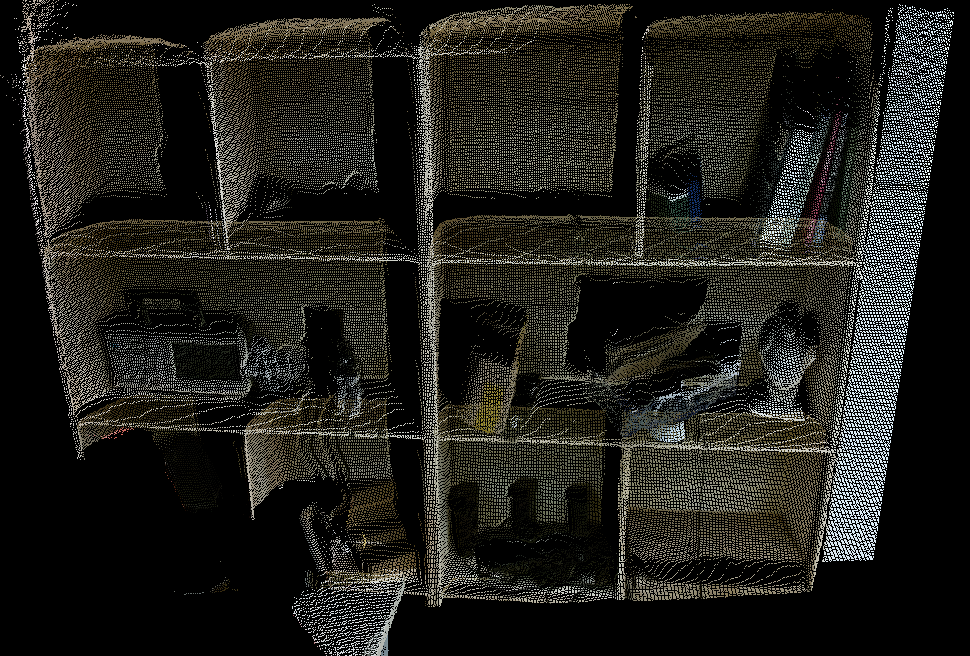
\includegraphics[width = 0.8\textwidth]{images/00.png}
    \caption{原始点云}
    \label{fig:initial_pc}
\end{minipage}
\begin{minipage}[t]{0.5\textwidth}
	\centering
    
\includegraphics[width = 0.9\textwidth]{images/01.png}
    \caption{确定的背景}
    \label{fig:bg}
\end{minipage}
\end{figure}

为了进一步清理RGB过滤中获取的信息,实现目标的准确定位,我们将利用目标图层和书架背景图层对应的三维模型进行深度信息的处理。\ 我们在书架背景图层中找到一个最大的平面作为墙面,以墙面的坐标为基准,去除目标图层中在那些在墙面上的点。\ 最后,我们对清理后的背景图层进行欧几里得聚类,将每一组几何关系上相互连接的点认作是一个目标,完成全部目标的定位工作。\ 

\begin{figure}[H]
\begin{minipage}[t]{0.5\textwidth}
	\centering
    
\includegraphics[width = 0.85\textwidth]{images/02.png}
    \caption{物体图层}
    \label{fig:obj}
\end{minipage}
\begin{minipage}[t]{0.5\textwidth}
	\centering
    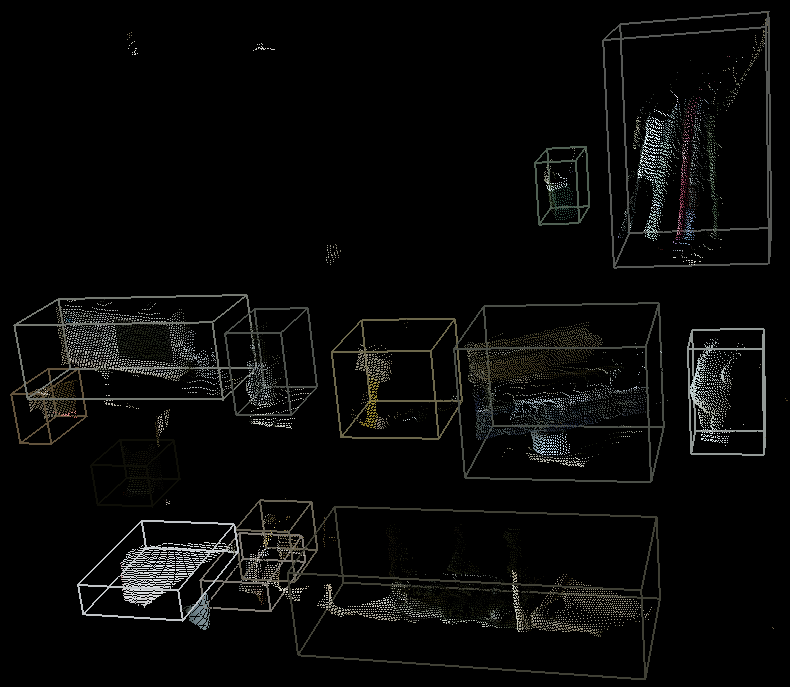
\includegraphics[width = 0.65\textwidth]{images/03.png}
    \caption{聚类后的物体图层}
    \label{fig:clustering}
\end{minipage}
\end{figure}

\begin{figure}[H]
\begin{minipage}[t]{0.5\textwidth}
	\centering
    
\includegraphics[width = 0.7\textwidth]{images/04alp.png}
    \caption{糖果袋}
    \label{fig:alp}
\end{minipage}
\begin{minipage}[t]{0.5\textwidth}
	\centering
    
\includegraphics[width = 0.45\textwidth]{images/05baymax.png}
    \caption{Baymax模型}
    \label{fig:baymax}
\end{minipage}
\caption{物体点云}
\end{figure}

\subsubsection{末端视觉}

我们从末端摄像头获得原始图像,其分辨率为$640\times480$,以$10$Hz的频率从摄像头读取,并且包装成ros信息后被发布,供后续模块读取。\ 正如上一部分所说,对于室内场景的图片,我们可以使用灰度熵来处理图像,对于末端视觉我们也采用了这种方法。\ 处理之后我们便获得了物体的图像,接着我们需要辨别物体的类型。\ 作为前提,我们不妨直接取所有物体中轮廓最大的那个作为研究的目标物体。\ 

\paragraph{物体识别}

我们使用 基于稀疏表示的分类器(Sparse Representation-based Classification)对上述的图像进行识别。\ 首先,我们事先准备该物体一定数量的样本,并假设当样本数量足够时,每张该物体的照片都可以近似表示为该物体样本照片的线性叠加,并且与其他物体的样本照片线性无关,这也就是“稀疏表示”的含义。\ 数学形式的表示为:
\begin{equation}
\boldsymbol{y} = A\,\boldsymbol{x_{0}} 
\end{equation}
其中$\boldsymbol{x_{0}} = [0, ..., 0, a_{i, 1}, ..., a_{i, n_{i}}, 0, ..., 0]$,若该物体属于第$i$类。\ 

可以证明\cite{wright2009robust},稀疏解$x_{0}$可以近似的被如下的表达式所估算:
\begin{equation}
\label{stable_l1}
\hat{x_{1}} = \text{arg}\ \text{min} ||\boldsymbol{x} ||_{1} \qquad\text{s.t.}\: ||A\boldsymbol{x}-\boldsymbol{y}||_{2} \leq \varepsilon 
\end{equation}

并且可以证明,$\hat{x_{1}}$能充分接近$\hat{x_{0}}$。\ 具体的实现方法如下:

\begin{enumerate}
\item 首先给定一系列样本矩阵$\mathbf{A}$,被测试样例$\boldsymbol{y}$,以及可容忍误差$\varepsilon$;
\item 将$\mathbf{A}$标准化使其有单位的$L_2$范数,然后求解方程\eqref{stable_l1};
\item 依次计算残差$r_{i}(\boldsymbol{y}) = ||\boldsymbol{y}-A\delta_{i}(\hat{x_{1}})||_{2}$,其最小值即为我们识别的结果。\ 
\end{enumerate}

\paragraph{降采样}

为了降低$\boldsymbol{y}$的维数,从而加快运算速度,对图片进行特征提取是很有必要的。\ 从数学上可以证明,只要提取的特征向量的维度大于$O( \log n)$,就不会影响方程\eqref{stable_l1}的解,因此我们可以直接对图片进行降采样。\ 

\subsubsection{机械臂设计}

\paragraph{结构设计思路}

选用的舵机能够负载$30$N$\cdot$m,舵机行程共$270^\circ$左右,动力充足,行程宽,故希望能够将舵机的有效行程缩短至所需的范围,以此优化机械臂的动力分配性能。

\paragraph{第一版}

如图\ref{fig:arm1}所示,第一版机械臂为兼容延续之前的机械设计以及成果,采用了较为灵活的钣金结构设计,沿用了前作的底座,有效的节省了设计周期与成本。

\begin{figure}[H]
    \centering
    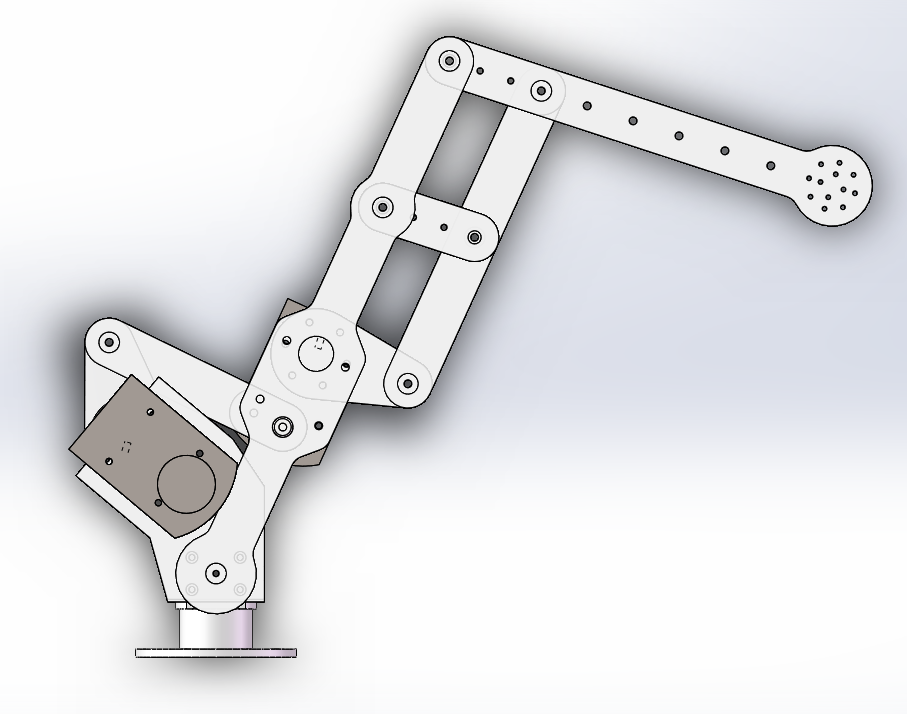
\includegraphics[width = 0.75\textwidth]{images/arm_1.png}
    \caption{第一版机械臂外观}
    \label{fig:arm1}
\end{figure}

在图\ref{fig:arm2}中可以看到有关机械臂的设计的原始尺寸,其主要目的为规划舵机的行程,使得行程充分转化,以达到优化的目的。

\begin{figure}[ht]
\begin{minipage}[t]{0.5\textwidth}
    \centering
    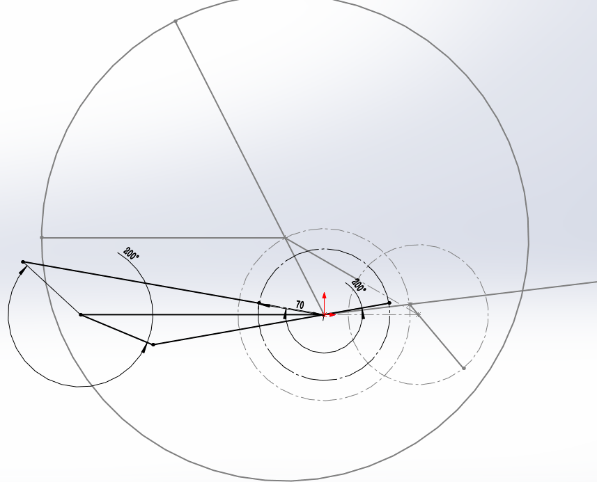
\includegraphics[width = 0.9\textwidth]{images/arm_2.png}
\end{minipage}
\begin{minipage}[t]{0.5\textwidth}
    \centering
    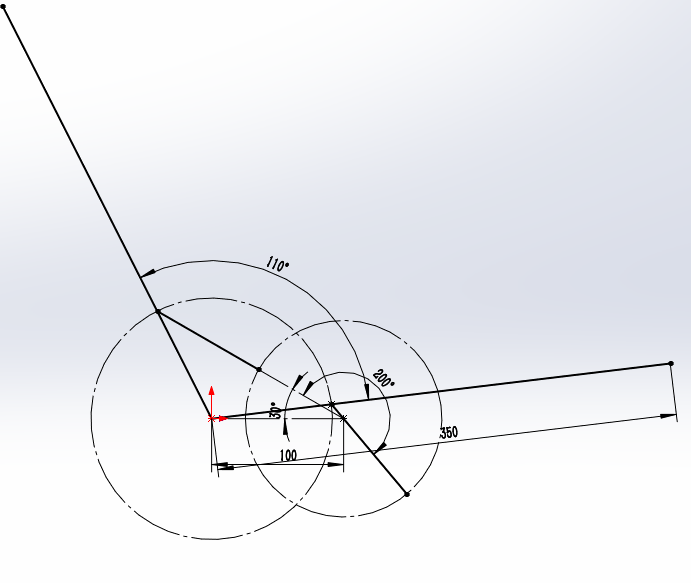
\includegraphics[width = 0.9\textwidth]{images/arm_3.png}
\end{minipage}
\caption{机械臂行程规划图}
\label{fig:arm2}
\end{figure}

如图\ref{fig:arm4}所示,第一版机械臂的载荷(蓝色)随机械臂上提而减小,同时机械臂的动力却在逐渐上升,从而在运动的中后段能够灵活有效的运动,但在前段会出现一段较大的动力不足的区间。

\begin{figure}[H]
    \centering
    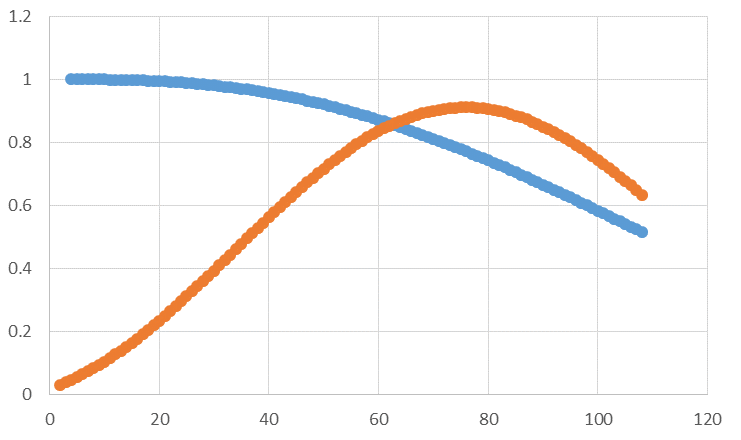
\includegraphics[width = 0.75\textwidth]{images/arm_4.png}
    \caption{第一版机械臂负载与载荷关系}
    \label{fig:arm4}
\end{figure}

第二版:如图\ref{fig:arm5}所示,第二版在前一版的基础之上加装了一个自由度,同时增加了许多的横向加固的内梁结构,能够有效的解决前一版机械臂抗扭曲刚度不足的问题。

\begin{figure}[H]
    \centering
    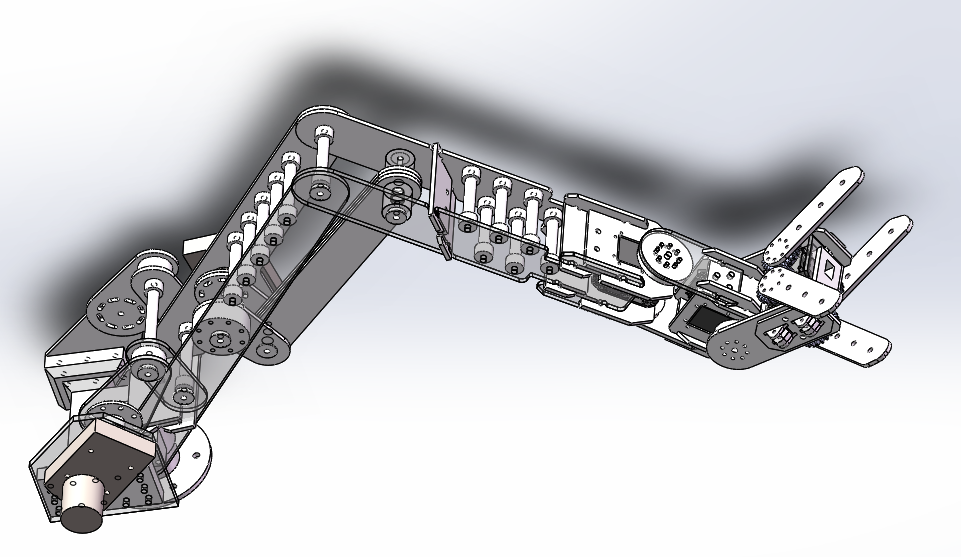
\includegraphics[width = 0.75\textwidth]{images/arm_5.png}
    \caption{第二版机械臂总成图}
    \label{fig:arm5}
\end{figure}

如图\ref{fig:arm6}所示,在第二版的机械臂设计中,吸取了上一版的机械臂的长处与优点,并且针对前一半的机械臂在前半段的运动区间内有较大的动力不足的情况作出了改进,改进后的载荷与负载关系如图\ref{fig:arm7}所示。

\begin{figure}[ht]
\begin{minipage}[t]{0.35\textwidth}
    \centering
    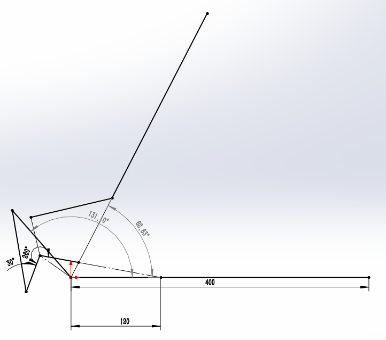
\includegraphics[width = 0.9\textwidth]{images/arm_6.png}
\end{minipage}
\begin{minipage}[t]{0.65\textwidth}
    \centering
    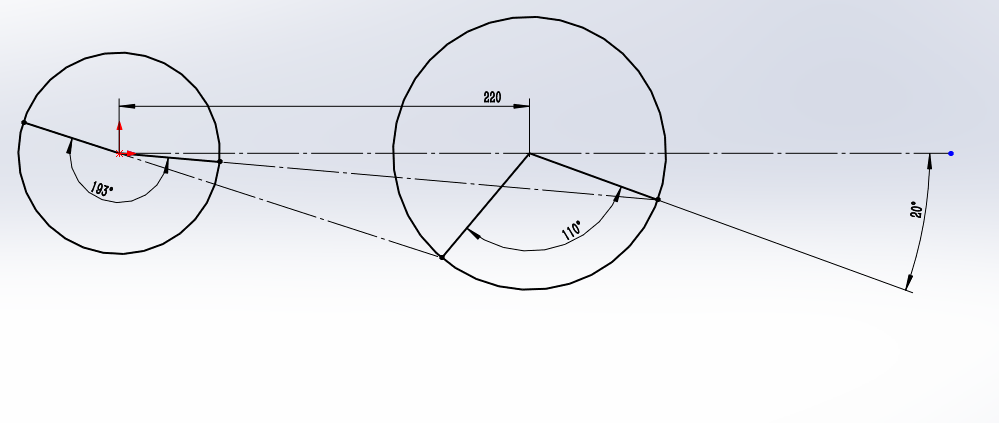
\includegraphics[width = 0.9\textwidth]{images/arm_7.png}
\end{minipage}
\caption{机械臂行程规划图}
\label{fig:arm6}
\end{figure}

\begin{figure}[H]
    \centering
    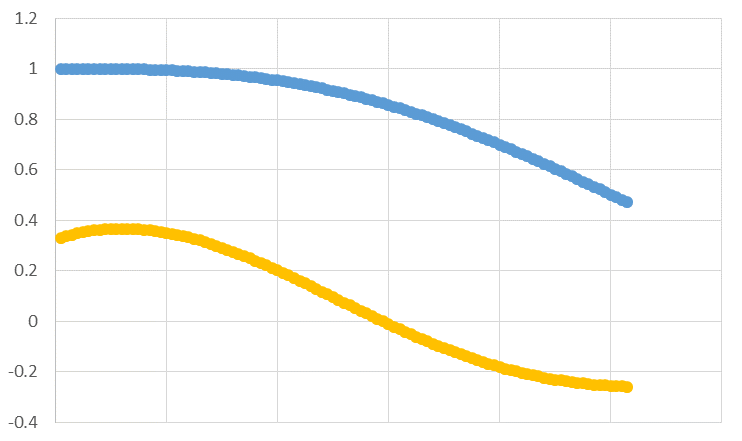
\includegraphics[width = 0.75\textwidth]{images/arm_8.png}
    \caption{第二版机械臂动力分配效果}
    \label{fig:arm7}
\end{figure}

\paragraph{其他创新设计}

在第二版的机械臂设计中,拟增加自适应机械手环节,使得$70$N$\cdot$m的舵机能够发挥充足的握力,拥有臂上一版更加优良的抓持稳定性,其自适应手结构目前仍在设计阶段,初期尺寸规划及行程安排如图\ref{fig:arm8}。

\begin{figure}[H]
    \centering
    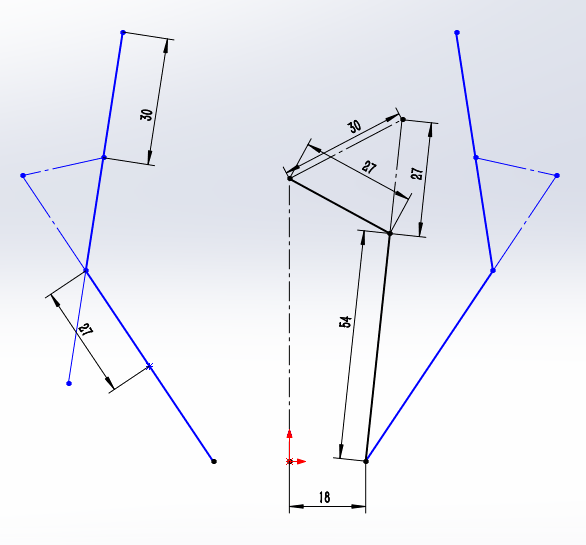
\includegraphics[width = 0.6\textwidth]{images/arm_9.png}
    \caption{自适应手关节初期设计草图}
    \label{fig:arm8}
\end{figure}

\subsubsection{机械臂控制}

考虑到控制算法的可扩展性,我们采用了通用的机械臂位姿算法。\ 首先,建立机械臂对象,输入机械臂每一段的转轴方向、相对于下一个关节的位移即可。\ 在建立了模型后,便可通过机械手的目标位置解算出电机的目标角度。\ 求解时采用了一种非线性优化算法,LM算法(Levenberg-Marquardt)\cite{more1978levenberg}。\ 它将高斯-牛顿法与梯度下降法相结合,从初始点开始迭代,通过合适的阻尼因子$\lambda$来达到最终解。\ 这个算法能够有效处理冗余参数的问题,在处理实际问题时效果良好。\ 

在具体的实现过程中,由于算法对初值敏感,所以我们会在机械臂当前角度作为初值求解失败后采用随机的角度作为初值重复求解直至得到结果。\ 

在每一次抓取物体之前,机械臂会回到初始位置,从深度视觉获得目标物体的三维位置信息作为机械手的初始目标。\ 机械手向前移动,在此过程中不断接收末端摄像头识别出的物体位置,依此在yz平面上调整目标位置,形成闭环控制。\ 距离传感器不断探测机械手与物体的距离,在到达阈值后让机械手上的电机转动,抓取物体。\ 

\begin{figure}[H]
    \centering
    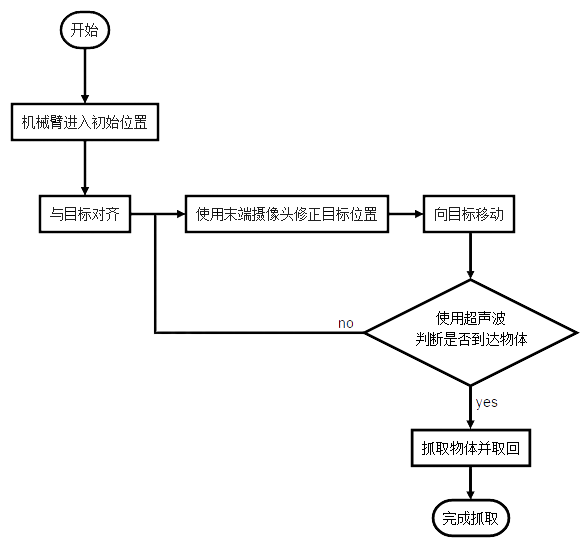
\includegraphics[width = 0.8\textwidth]{images/arm.png}
    \caption{机械臂流程图}
    \label{fig:arm}
\end{figure}

另外,为了保证深度视觉信息的准确,在Kinect2获取场景图像前,机械臂将旋转至一个边缘位置,到Kinect2的视野之外,减小对于图像与深度信息的干扰。\ 

\subsubsection{距离传感器}

由于单目的末端摄像头无法准确获得物体的深度信息,通过深度视觉获取的深度信息精度也无法保证,所以我们在机械手上加装了末端超声波传感器,用来准确探测与目标物体之间的距离。\ 在距离达到阈值后,便告知机械臂已到达目标位置,可以开始抓取物体。\ 

\subsubsection{移动底盘}

在底盘设计中,原本采用四个独立正交的欧姆尼轮作为运动输出,但在实际使用过程中发现该设计的通过性较弱,不能够适应复杂的环境,容易被线缆等物体牵制。故在后续的设计中,我们采用麦克纳姆轮作为动力输出,使得底盘能够在保持全向运动性的同时获得更大的带载能力与更好的通过性。

\begin{figure}[ht]
\begin{minipage}[t]{0.35\textwidth}
    \centering
    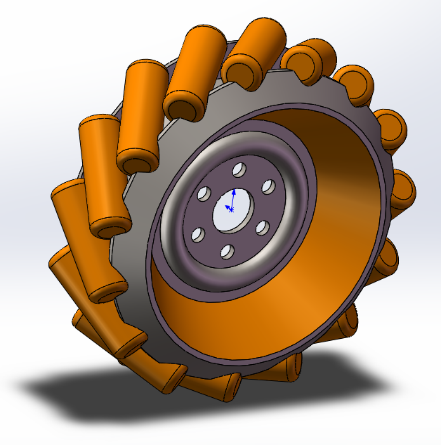
\includegraphics[width = 0.9\textwidth]{images/chassis_1.png}
\end{minipage}
\begin{minipage}[t]{0.65\textwidth}
    \centering
    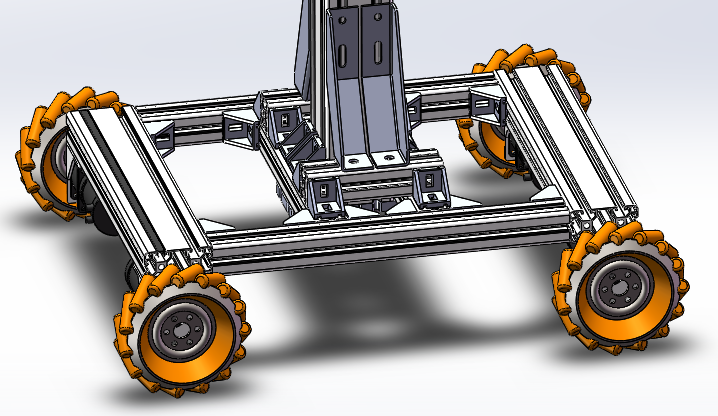
\includegraphics[width = 0.9\textwidth]{images/chassis_2.png}
\end{minipage}
\caption{麦克纳姆轮及底盘}
\label{fig:cha1}
\end{figure}

同时,在新的底盘设计设计中,采用了6063铝型材作为底盘的主框架,有效的增加了底盘的可扩展性与比强度,简化了设计的难度。

\begin{figure}[H]
    \centering
    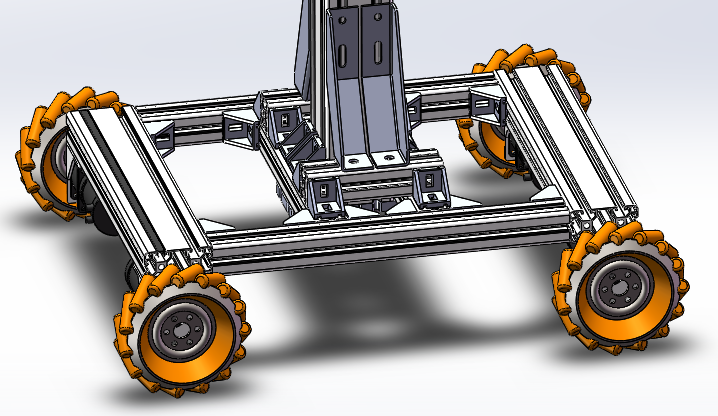
\includegraphics[width = 0.6\textwidth]{images/chassis_2.png}
    \caption{选用的欧标6063铝型材横截面示意图}
    \label{fig:cha2}
\end{figure}



\section{项目成果}

\subsection{实物图片}

\begin{figure}[H]
    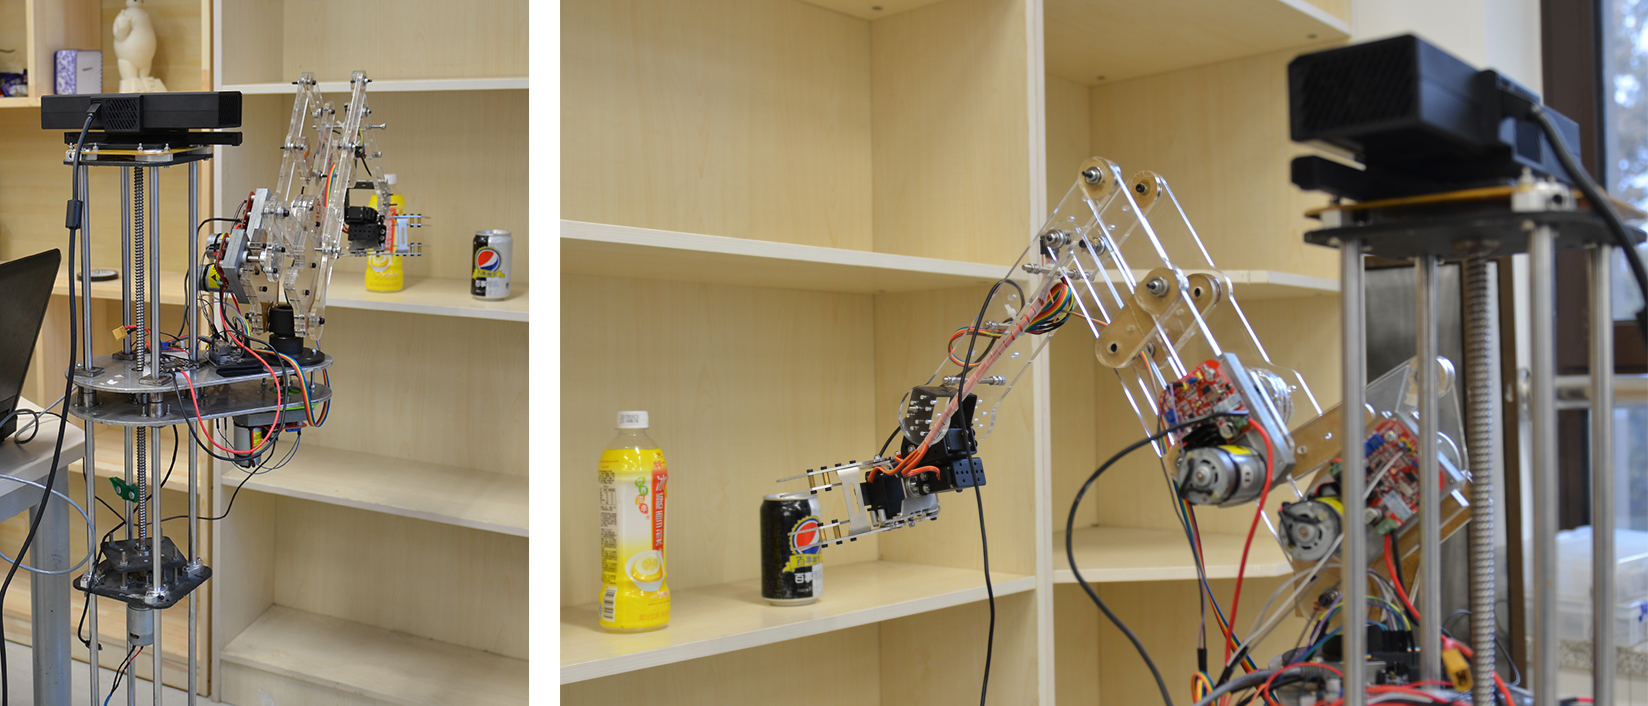
\includegraphics[width = \textwidth]{pictures/1.png}
    \caption{第一版机械臂实物图}
    \label{fig:1}
\end{figure}

\begin{figure}[H]
    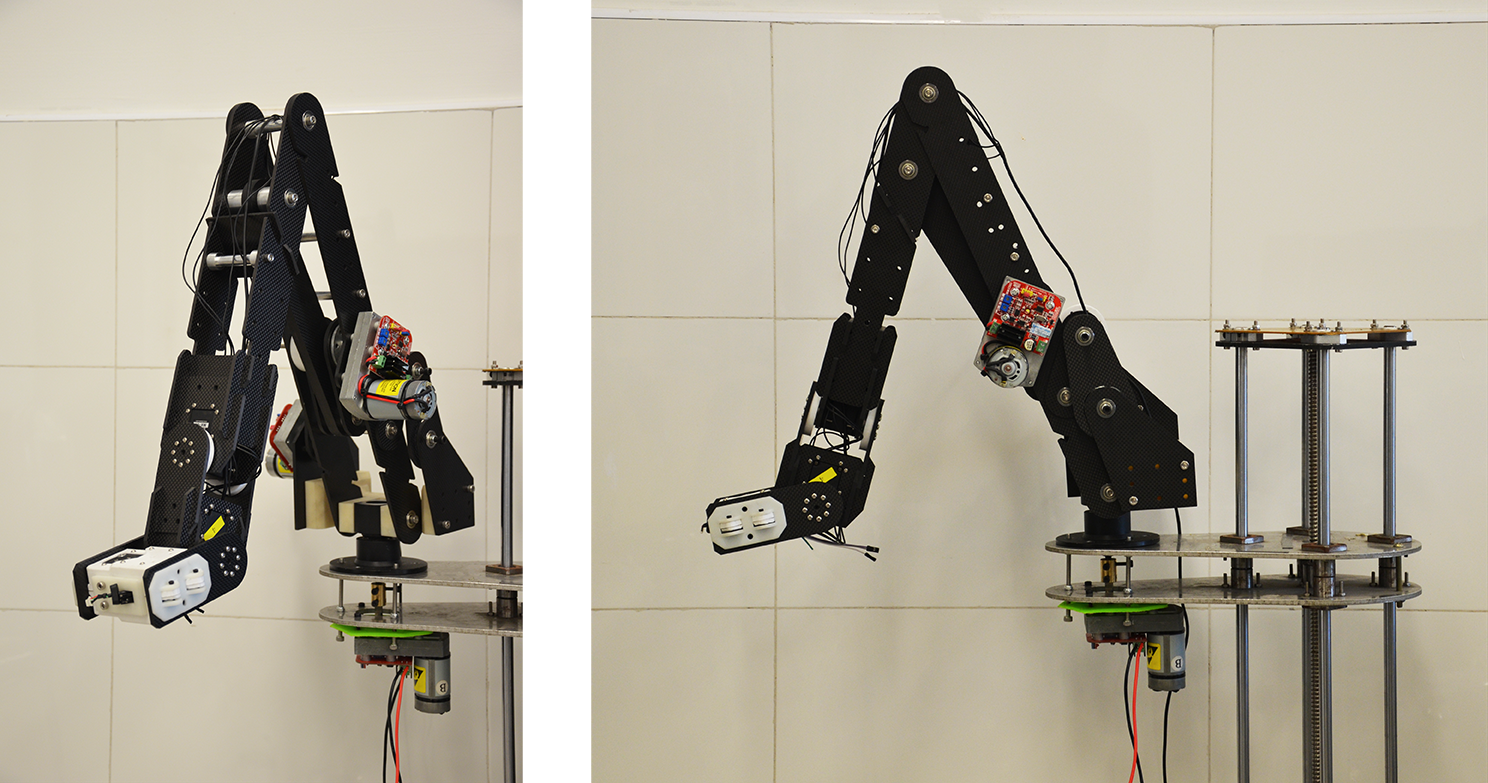
\includegraphics[width = \textwidth]{pictures/2.png}
    \caption{第二版机械臂实物图(仍在制作中)}
    \label{fig:1}
\end{figure}
\subsection{测试结果}

图像处理的测试结果见图\ref{fig:registered},\ref{fig:entropy_block},\ref{fig:downsampled_filled},\ref{fig:color_block},\ref{fig:raw_contour},\ref{fig:after_contour},\ref{fig:final_contour},\ref{fig:lines}所示。

立体视觉获得的点云处理结果如图\ref{fig:initial_pc},\ref{fig:bg},\ref{fig:obj},\ref{fig:clustering},\ref{fig:alp},\ref{fig:baymax}所示。

物体识别的测试结果见图\ref{fig:du1}, \ref{fig:du2}。图\ref{fig:du1}中,左侧窗格显示的sci代表相似度,name代表识别出的物体。

\begin{figure}[H]
    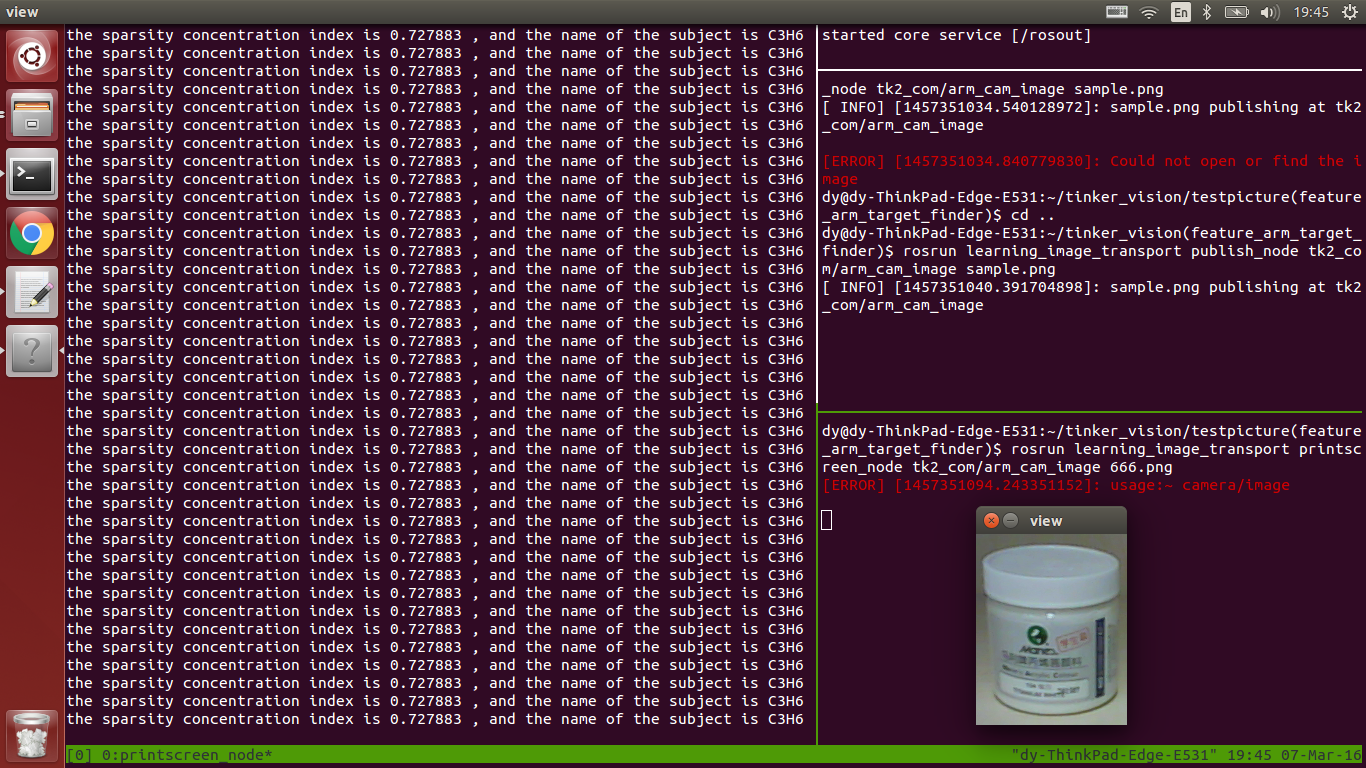
\includegraphics[width = \textwidth]{images/du1.png}
    \caption{物体识别结果}
    \label{fig:du1}
\end{figure}

\begin{figure}[H]
    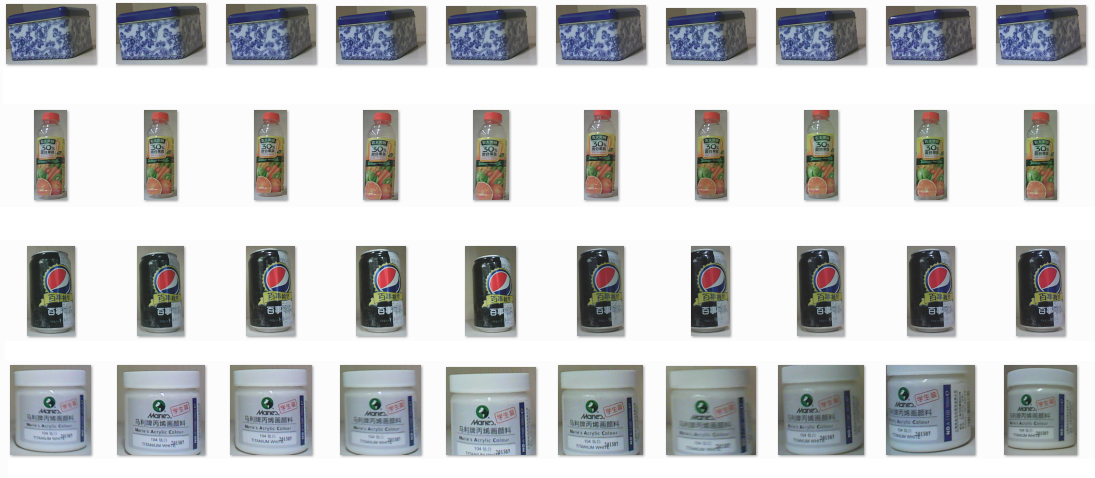
\includegraphics[width = \textwidth]{images/du2.png}
    \caption{物体样本库}
    \label{fig:du2}
\end{figure}

整个系统经测试后能够良好的完成物体定位、识别与抓取任务,具体过程请见视频附件。

\section{发展前景与应用价值}

我们的机械手能够准确的识别物体并抓取,填补了目前家庭机器人市场中缺乏物体移动功能的空缺。在具有了识别并抓取物体的能力后,机械手能够完成许多基本而有必要的家居任务,比如从柜子上取下一个指定的东西送到手边,或者把桌上杂乱的物体排列整齐,在实际的日常生活中也具有较大的应用价值。

\section{总结}

\subsection{项目进展}

目前,我们的项目已经调试通过了所有模块,也在联合调试中测试了整体的性能。\ 我们的机械臂能够准确的识别物体并抓取,最后将其放在指定的地方,达到了预期效果。\ 现在,我们已经根据第一版机械臂的不足设计制造了第二版机械臂,将在之后的一个月内进行调试。项目进度见表\ref{tab:progress}。

\renewcommand\arraystretch{1.2}
\begin{table}[H]
\centering
\begin{tabular}{l|c}
\hline
时间 & 进度 \\ \hline
2015.9-2015.10 & Kinect测试 \\
 & Kinect物品识别算法开发 \\ \hline
2015.11 & 项目立项,进行可行性分析 \\ \hline
2015.12 & 电机选型、购买与测试 \\ \hline
2016.1 & 初版机械臂设计与加工 \\
 & 机械臂控制算法开发 \\
 & 末端摄像头物品识别算法开发 \\ \hline
2016.3 & 第二版机械臂设计与加工 \\
 & 加入移动平台 \\ \hline
\end{tabular}
\caption{项目进度}
\label{tab:progress}
\end{table}

\newpage

\subsection{展望}

我们的系统还有若干方面有改善与提高的空间。\ 我们希望增加机械手的自由度,配合图像算法,使其能够从最合适的方向抓取物体,增加在实际场景中的适应能力;使用如激光雷达来知周围的环境,让我们的机械臂能够更加灵活自主的在房间中移动;语音系统与人脸识别系统,让机械臂能够与人更好的交互。

希望我们的机械臂能走近更多的家庭,帮助人们分担更多的家务,让人们的家居生活更加简单轻松。


\bibliographystyle{unsrt}
\bibliography{bibfile}

\end{document}